\documentclass[12pt]{article}
\usepackage{graphicx}
\usepackage{fullpage}
\usepackage{float}
\usepackage[symbol]{footmisc}
\graphicspath{{../images/}}

\title{Lab 1: The Analog Lab}
\author {
Kevin Yu
}

\begin{document}
\maketitle

\begin{abstract}
We study the properties of basic analog circuit components, and demonstrate how they can be used to filter and manipulate electrical signals. This culminates in the construction of an FM receiver capable of demodulating and amplifying a frequency modulated signal carried at $1.045MHz$. Additionally, we use our new understanding of impedances mismatches and reflections to estimate the length of a long cable. We measure the cable to be roughly $120m$, and the characteristic impedance of the cable to be about $56\Omega$. Finally, we study sources and characteristics of noise in analog circuits, as well as how to determine the noise figure of an amplifier. To learn how to describe noise, we empirically verify the Central Limit Theorem (CLT), finding that the standard deviation of the sample average of $n$ measurements is proportional to $n^{-0.51\pm0.02}$, in agreement with the CLT prediction of $\sigma \propto n^{-0.5}$. Figures and code can be found online at http://github.com/kevinyu/astro121.git.
\end{abstract}

\section*{Introduction}
In this first lab, we will learn to understand and manipulate radio signals using analog circuits. Understanding impedance will help us build frequency dependent filters so that we can extract the information we want from signals while excluding unwanted noise. We will learn the importance of impedance matching, where a mismatch in impedance can cause one section of a circuit to significantly alter the behavior of another or cause distortive effects due to reflections on a transmission line.

We will demonstrate these tools by building a FM Receiver, which will take a frequency modulated (FM) signal and convert it into a signal that we can listen to on a speaker. This will take advantage of LC and RC filters, DC biasing, and NPN transistors to help us amplify our signal. We will learn general techniques to optimize circuits such as proper termination, as well as ways we can characterize random noise in our results.

Because the purpose of this lab was to demonstrate understanding of basic components of analog circuits, the upcoming Theory section contains discussion of topics at a level which may bore the reader. If thats the case, please skip such sections and just assume I know what I'm talking about\footnote{this is in general not the case, but it'll be for the best if you go along with it}.

\section*{Theory}

\subsection*{Impedance}
Impedance is a generalization of resistance that, through Ohm's Law $V=IR$, relates the current through a conductor to the voltage across it. In the case of capacitors and inductors, impedances can be both complex and frequency dependent. The impedances of resistors, capacitors, and inductors are:
\begin{eqnarray}
Z_{resistor} &=& R\nonumber\\
Z_{capacitor} &=& (j\omega C)^{-1} \nonumber \\
Z_{inductor} &=& j\omega L \nonumber
\end{eqnarray}
As you can see, capacitors have high impedances for low-frequency and DC signals, but have low impedance for high-frequency signals. Conversely, inductors oppose high-frequency signals while pass through low-frequency and DC signals.

Impedances add in the same way that resistances do.
\begin{eqnarray}
Z_{series} &=& \sum_i{Z_i}\nonumber\\
\frac{1}{Z_{parallel}} &=& \sum_i{\frac{1}{Z_i}}\nonumber
\end{eqnarray}
For example, equivalent resistance of an infinite row of resistors in parallel (the question posed in the lab manual) is:
\begin{eqnarray}
\frac{1}{Z_{eq}} &=& \sum_\infty\frac{1}{R} \rightarrow \infty \nonumber \\
Z_{eq} &=& 0\nonumber
\end{eqnarray}

As an example of adding frequency dependent and complex impedances, Figure \ref{fig:LCimpedances} shows the impedance of an inductor and capacitor combined in series and in parallel at different frequencies.

\begin{figure}[H]
\center{
  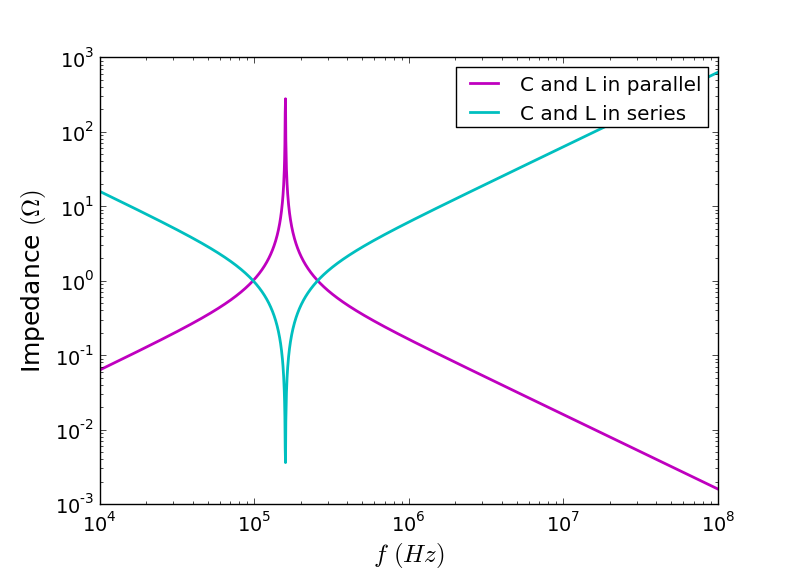
\includegraphics[width=360px]{LC_parallel_series}
}
\caption{Impedance of an inductor and a capacitor connected in parallel and in series. At the frequency $\omega_0=\frac{1}{\sqrt{LC}}$, the impedance of the two in series goes to zero, while the impedance of the two in parallel becomes infinitely large (this is at the LC circuit's resonant frequency). This response is utilized in our bandpass filter.}
\label{fig:LCimpedances}
\end{figure}

\subsection*{Reflections and Termination}
At the interface between two transmission lines with different impedances, a signal can be partially, or entirely, reflected back from whence it came. When a signal reaches an interface going from low impedance to high impedance (for example, terminated with open circuit), the signal will be reflected with no inversion. At an interface from high impedance to a low impedance (for example, terminated with a short), the signal will be reflected and inverted. 

If the time delay between the a signal and its reflection is measured, we can convert that into the time it takes the signal to travel up and back down the wire and solve for the length of the cable, using\footnote{Approximating the speed of signal propogation in the cable to be $\frac{2}{3}c$}:

\begin{eqnarray}
l_{cable} = \frac{2c}{3} \frac{\Delta{t}_{delay}}{2} \label{eq:cablelength}
\end{eqnarray}

To get rid of reflections, which can distort a signal, the cables should be properly terminated with an impedance matching the characteristic impedance of the cable itself, which will minimize unwanted reflections.

\subsection*{Voltage Divider}
A basic use of impedances is the voltage divider. A voltage divider, depicted in Figure \ref{fig:voltagedivider}, obeys the following relationship, which can be derived directly from Ohm's law, $V=IZ$.
\begin{eqnarray}
V_{out} = \frac{Z_2}{Z_1+Z_2} V_{in} \label{eq:voltagedivider}
\end{eqnarray}
\begin{figure}[H]
\center{
  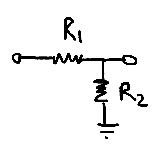
\includegraphics{volt_divider}
}
\caption{Voltage divider, shamelessly stolen from the lab manual.}
\label{fig:voltagedivider}
\end{figure}

\subsection*{RC Filter}
One application of a voltage divider is an RC filter. An RC filter is a voltage divider consisting of a resistor and a capacitor. A high-pass filter involves a capacitor connecting input to output and a resistor connecting output to ground; in Eq.\ref{eq:voltagedivider}, it corresponds to $Z_1=Z_C$ and $Z_2=R$. A high-pass filter lets through high frequency signals because for large $\omega$, $|Z_C| \ll |Z_R|$ and $Gain\footnote{Gain defined as $V_{out}/V_{in}$} \rightarrow 1$. For low frequency signals, $|Z_C| \gg |Z_R|$ and $Gain \rightarrow 0$, meaning the signal will be completely attenuated.

A low-pass filter is similar to the high-pass filter, with the positions of the capacitor and resistor reversed. Through similar arguments at high and low frequency limits, the gain goes to $1$ at low frequencies and goes to $0$ at high frequencies.

In both the high-pass and low-pass cases, there is a frequency at which the power output of the voltage divider is halved; i.e. $(V_{out}/V_{in})^2 = 0.5$. In decibels (dB)\footnote{decibels are defined as $20\log_{10}{(V_{out}/V_{in})}$}, this is the $-3dB$ point. In RC filters, this occurs at the roll-off frequency
\begin{eqnarray}
\omega = \frac{1}{RC}\label{eq:rolloff}
\end{eqnarray}
A dramatic portrayal of the response of high-pass and low-pass filters can be seen in Figure \ref{fig:highandlowpass}.
\begin{figure}[H]
\center{
  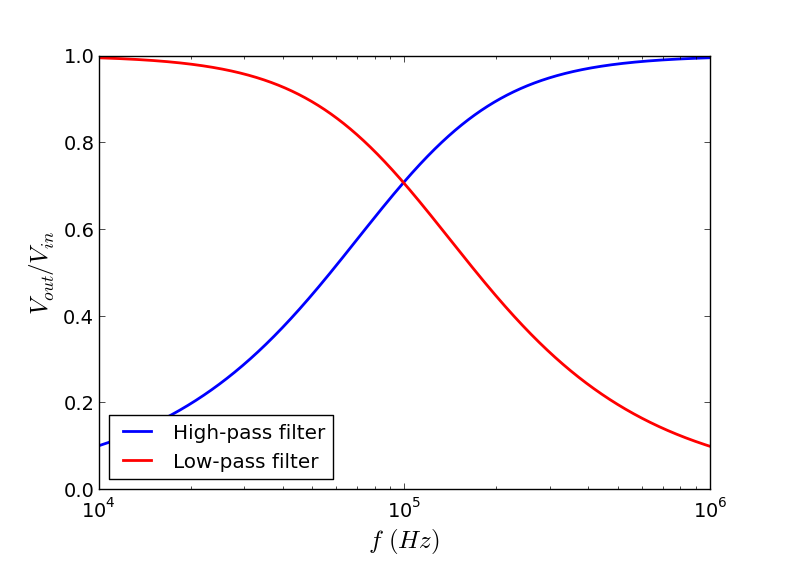
\includegraphics[width=360px]{RC_High_and_Low_pass}
}
\caption{Theoretical transfer functions for RC high-pass and low-pass filters with the same roll-off frequency of $10kHz$.}
\label{fig:highandlowpass}
\end{figure}
\subsection*{FM Demodulator}
We will be using the above to build a circuit capable of receiving a frequency-modulated signal and extracting the underlying signal. The modulated carrier wave will be a frequency a few orders of magnitude higher than the modulating signal. In this section I will describe how the demodulation works, referring to the circuit diagram in Figure \ref{fig:fmdemoddiagram} for each separate section.
\begin{figure}[H]
\center{
  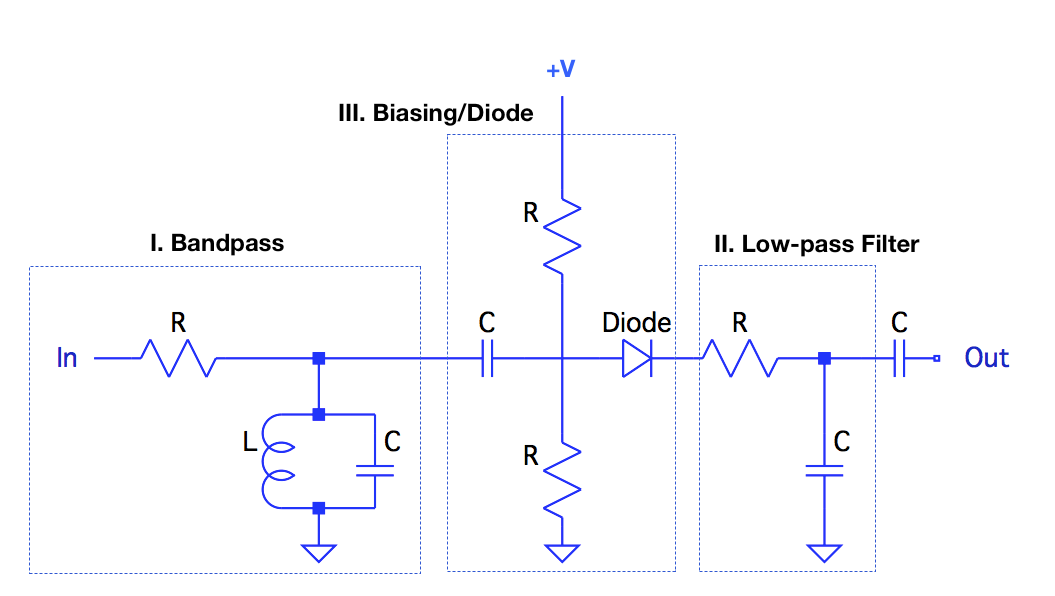
\includegraphics[width=360px]{fmdemod_diagram}
}
\caption{Depiction of the FM Demodulator.}
\label{fig:fmdemoddiagram}
\end{figure}

\subsubsection*{I. LC Bandpass Filter}
A capacitor and inductor can be combined in parallel to create a bandpass filter, a filter which only passes signals in a certain frequency range unattenuated. It is done by taking advantage of the behavior of an inductor and capacitor in parallel (Figure \ref{fig:LCimpedances}) near the resonant frequency of an LC loop,
\begin{eqnarray}
\omega_0 = \frac{1}{\sqrt{LC}} \label{eq:resonantfrequency}
\end{eqnarray}
The LC bandpass filter that we will create is a voltage divider with a resistor connecting the input to output, and an inductor and capacitor, in parallel, connecting the output to ground.

Referring to the notation in Eq.\ref{eq:voltagedivider}, the voltage divider will have an extremely large $Z_2$ at frequencies near the resonant frequency, leading to little attenuation, while having a small $Z_2$ farther from the resonant frequency, leading to significant attenuation. The end result is that only frequencies near the resonant frequency get passed through unattenuated.

The resistor, $Z_1$ in this case, determines the bandwidth of the filter; it affects how far from resonance a signal must be before $Z_2 \approx Z_1$. The width of the bandpass can be defined in terms of the same $-3dB$ level of attenuation used in the earlier RC section:
\begin{eqnarray}
\Delta{f}_{-3dB} &=& \frac{f_0}{Q}\label{eq:bandwidth}\\
Q &=& R\sqrt{\frac{C}{L}}\nonumber
\end{eqnarray}

The purpose of this bandpass filter in the context of our demodulator is to differentially attenuate frequencies in the FM modulation span. By tuning the resonant frequency of the bandpass to a value slightly below the center carrier frequency, and choosing the right $Q$, we can have the carrier wave's frequencies span the downward sloped region of the bandpass filter's response. This can be seen in Figure \ref{fig:bandpasstransfer}; higher frequency sections of this signal will have decreased amplitudes; this converts the frequency modulated signal into an amplitude modulated (AM) signal.

\subsubsection*{II. Low-pass Filter}
The objective after converting the signal to AM is to extract the ``envelope" by removing the high frequency carrier wave---leaving only the lower frequency (audible) signal behind. To do this, we can use a low-pass filter. Because the capacitor in the low-pass filter responds slowly to high frequency changes, by picking a filter with a roll-off below the carrier frequencies we essentially will average out the carrier wave. However, we still want to preserve the amplitude information. This poses a problem because the signal spends an equal amount of time below and above zero, and a slow time constant in the low-pass filter will average the signal out to zero---the amplitude information will be lost! To fix this, we will use a diode.

\subsubsection*{III. Biasing and Diode}
A diode is a component that only conducts current in one direction if the voltage across it exceeds a critical value (in our case, it will be about $0.6V$). Once conducting, the voltage drop across the diode stays at a constant value unless the signal drops back down below $0.6V$, in which case it will no longer conduct.

In the last section, we saw that we needed a way to preserve the amplitude information when smoothing over our signal. To do this, we will only allow the positive half of the AM signal to propogate, blocking out the negative half. This way, instead of having the low-pass filter average out both positive and negative, which will come out to zero, if we only average the positive half of the signal the low pass filter will smooth out the carrier wave but leave the relative amplitude information of the envelope intact.

We will choose biasing resistors in the voltage divider such that Eq.\ref{eq:voltagedivider} gives us a biasing voltage of about $0.6V$. Note that the coupling capacitor right before the voltage divider ensures that there is no DC bias onther than the bias we provide here. When an AC signal is added on top of this bias, the diode will only conduct the positive half of the AC signal.

\subsection*{Amplifier}
\begin{figure}[H]
\center{
  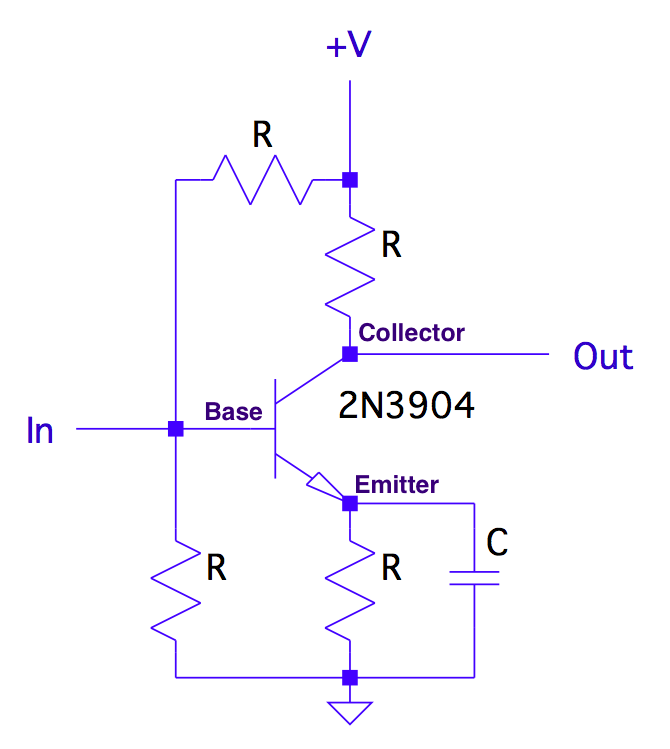
\includegraphics[width=150px]{amplifier_diagram}
}
\caption{BJT Amplifier.}
\label{fig:amplifier_diagram}
\end{figure}

To increase the amplitude of the signal, we will use the NPN BJT amplifier in Figure \ref{fig:amplifier_diagram}. The BJT conducts current through the collector to the emitter as long as the voltage drop from the base to the emitter is above a certain voltage, $V_{BE}$ (for us it will be very close to $0.6V$). This voltage is in equilibrium and thus setting the base voltage fixes the emitter voltage. If the base-emitter voltage is greater than that threshold, more current will be drawn through the emitter resistor and the emitter voltage will rise until it reaches that $V_{BE}$. If the base-emitter voltage drops below $V_{BE}$, the transistor stops conducting and the emitter voltage drops until the equilibrium $V_{BE}$ is restored.

The gain of the amplifier can be set by the ratio of the collector resistor to the emitter resistor. This gain can be made frequency dependent by including capacitors in parallel with either resistor.
\begin{eqnarray}
g = \frac{R_{collector}}{R_{emitter}} \label{amplifiergain}
\end{eqnarray}
The current going through the emitter---and thus the collector---can be chosen by first figuring out the corresponding emitter voltage using Ohm's Law: $V_{emitter}=IR_{emitter}$. Then, since we know that the emitter voltage is fixed relative to the base voltage, we can choose biasing resistors so the voltage at the base is
\begin{eqnarray}
V_{base} = V_{emitter} + V_{BE} = V_{emitter} + 0.6V \label{vbase}
\end{eqnarray}

We can set the current through the emitter by choosing a base voltage such that it fixes $V_{emitter} = IR_{emitter}$, by choosing
\begin{eqnarray}
 \frac{V_{base} - 0.6V}{R_{emitter}} = I \label{eq:setcurrent}
\end{eqnarray}

\subsection*{Follower}
\begin{figure}[H]
\center{
  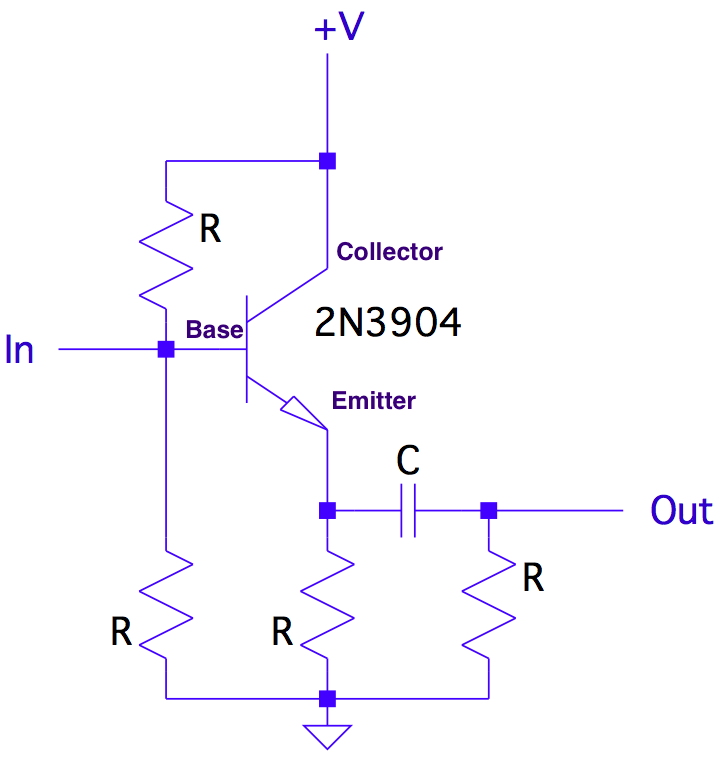
\includegraphics[width=150px]{follower_diagram}
}
\caption{BJT Emitter-Follower.}
\label{fig:follwer_diagram}
\end{figure}
Similar to the NPN BJT Amplifier, the follower is like an amplifier with a gain of 1. The transistor works in the same way that it works in the amplifier---the emitter voltage is held fixed at a voltage $V_{BE}$ lower than the voltage at the base. We can choose the two biasing resistors to be equal, so that the center voltage of the follower is halfway between GND and the power source voltage. The purpose of the emitter resistor is to set the current; this is possible becuase $V_{emitter}$ is fixed relative to $V_{base}$. Because the transistor cannot conduct if the base-emitter or collector-base are reverse biased, the selection of the bias at the base limits the amplitude of the signal that can be passed through the follower:
\begin{eqnarray}
V_{max,base} &=&V_{powersource}\label{eq:maxbase}\\
V_{min,base} &=& V_{center} - V_{BE}\label{eq:minbase}
\end{eqnarray}
The advantage of the emitter-follower is that it can isolate two different parts of a circuit from each other by matching input and output impedances. If we connect something with a small input impedance, such as our $8\Omega$ speaker, to an amplifier with a high ouput impedance directly, almost all of the voltage drop will occur across the amplifier and the speaker will receive very little current. The follower however holds the emitter voltage steady by design, regardless of the load. Rather than decrease the emitter voltage, a small load will tend to draw more current from the power source in order to keep it at a steady potential relative to the base. The follower matches impedances with a large input impedance and a small output impedance.
\subsection*{Noise}
\subsubsection*{Noise Factor}
The power added to a circuit due to Johnson-Nyquist noise, caused by the random thermal motion of electrons in a resistor, is described by
\begin{eqnarray}
\frac{P}{B} = k_B T \label{johnsonnyquist}
\end{eqnarray}
The noise figure of a circuit is defined as
\begin{eqnarray}
NF = 10\log_{10}{\frac{T_0 + T}{T_0}} \label{eq:noisefigure}
\end{eqnarray}
where $T_0=290K$. To determine the noise temperature of our amplifier, we can measure the noise power for a parcitular bandwidth, and use Eq.\ref{johnsonnyquist} to get $T$.

\subsubsection*{Central Limit Theorem}
The Central Limit Theorem (CLT) says that the distribution of a sample average of a random variable is gaussian, regardless of the distribution of the random variable itself. That is, if we record the average, $\bar{x}$, of $n$ measurements on a random variable $x$, the distribution of measurements of $\bar{x}$ should be gaussian around the true mean.

Additionally, the standard deviation of that gaussian distribution scales by the inverse squareroot of $n$. The more elements in the sample, the narrower the distribution is, and the closer the measurements of the average will be to the true mean. A demonstration of this relationship
\begin{eqnarray}
\sigma_{\bar{x}} \propto n^{-1/2} \label{eq:rootn}
\end{eqnarray}
is made in Figure \ref{fig:n_scaling}. The CLT can be used to characterize variations in a signal as random noise, as opposed to systematic errors.
\newpage
\section*{Methods}

\subsection*{FM Receiver}
In this Lab, we will build an receiver tuned to a FM carrier frequency centered at $1.045MHz$.

\begin{figure}[H]
\center{
  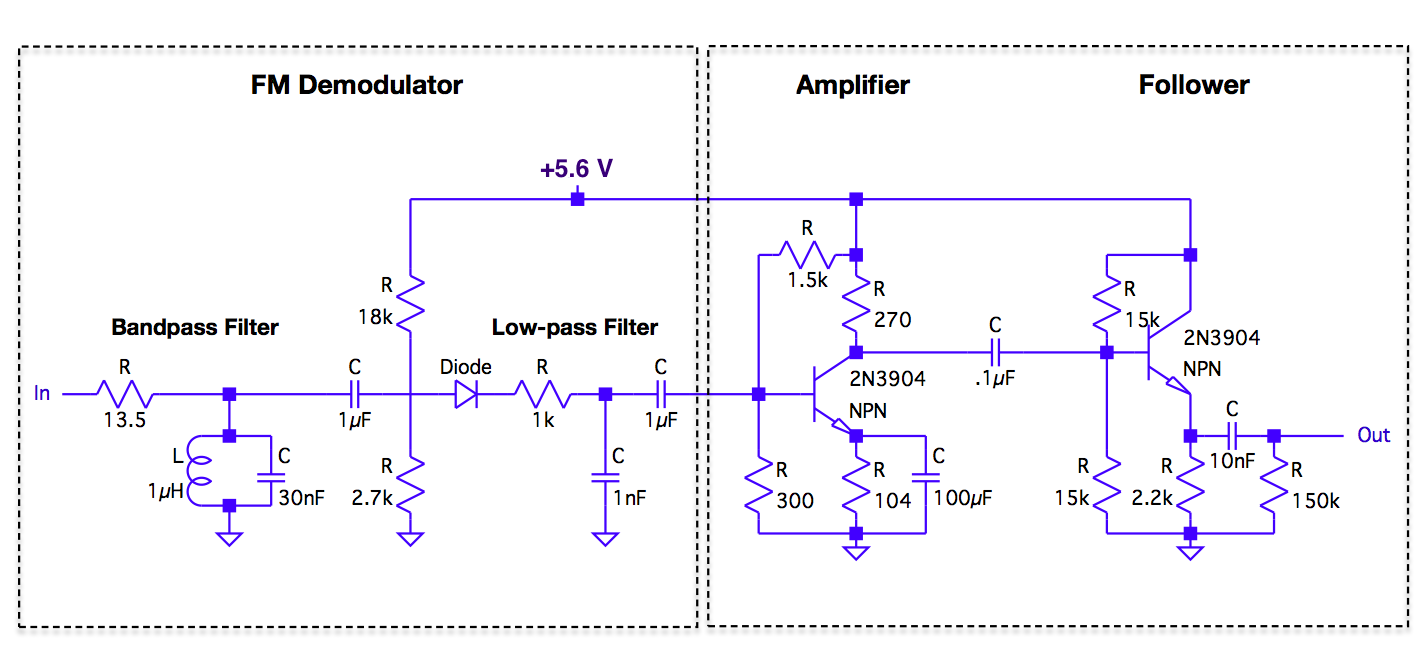
\includegraphics[width=480px]{Circuit_diagram_labeled_and_cropped}
}
\caption{Circuit diagram of our FM Receiver, with our selected component values. It consists of a FM demodulator connected in series with an amplifier and an emitter-follower.}
\label{fig:circuitdiagram}
\end{figure}

\subsubsection*{Building the FM Demodulator}
The first part of the FM Demodulator is the bandpass filter. As we discussed in the earlier section, we want to tune our LC bandpass filter to be centered at a frequency slightly below the carrier frequency, and to choose a bandwidth that gradually attenuates higher frequencies so we can differentiate the frequency modulations. Using Eqs. \ref{eq:resonantfrequency} and \ref{eq:bandwidth}, we chose values

\begin{center}
  \begin{tabular}{ c  c }
    L & $1\mu H$ \\
    C & $30nF$ \\
    R & $13.5\Omega$ 
  \end{tabular}
\end{center}
giving us a resonant frequency of $f_0 = 0.92 MHz$ and a bandwidth of $\Delta{f}_{-3db} = 0.39 MHz$. We chose the inductor because we have a very limited selection of components in the lab. For the resistor, we used two $27\Omega$ resistors in parallel, and for the capacitor we used three $10nF$ capacitors in parallel.

The response of this bandpass filter is shown in Figure \ref{fig:bandpasstransfer}, which illustrates how the FM signal will be attenuated at various levels over its frequency range.

\begin{figure}[H]
\center{
  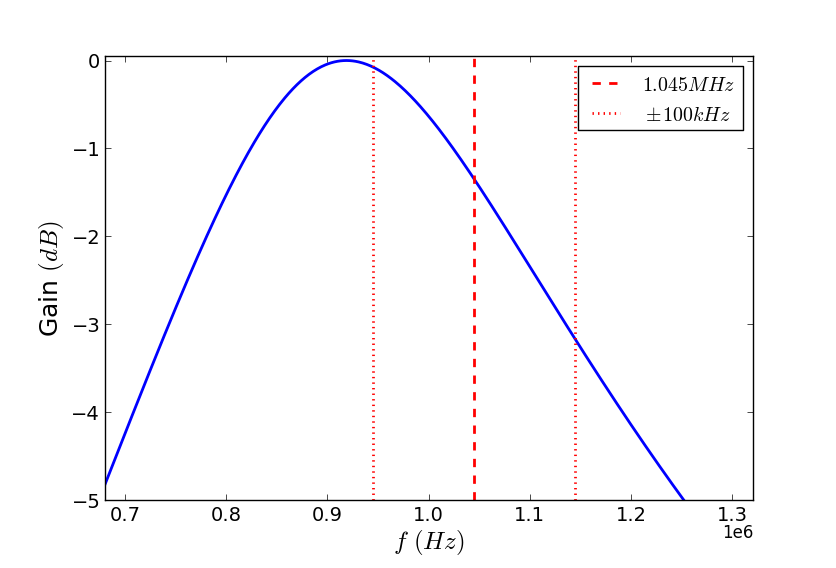
\includegraphics[width=360px]{FM_Reciever_Bandpass_In_dB}
}
\caption{Transfer function of our bandpass filter for $R =13.5\Omega$, $L=1\mu H$, $C=30nF$. This filter has a quality factor of $Q=R\sqrt{\frac{C}{L}}=2.34$ and a bandwidth of $\Delta f_{-3dB}=\frac{f_0}{Q}\approx 390kHz$. The range of carrier wave frequencies of our station lie in the downward sloping region of the transfer function, resulting in an amplitude modulated signal.}
\label{fig:bandpasstransfer}
\end{figure}

To bias the signal properly so that the positive half of the signal would pass through the diode and the negative half would be blocked, we needed to add a DC bias to the signal of $0.6V$. We chose the biasing resistors to be $18k$ (to the power supply) and $2.7k$ (to ground), and had our power supply set to $5.6V$. Using Eq.\ref{eq:voltagedivider}, our DC bias is $0.72V$, just above our desired voltage.

The low-pass filter needs to be able to smooth out the $1.045MHz$ carrier wave while leaving the underlying audio signal intact. To do this, we want a roll-off frequency somewhere between $\sim 1MHz$, the carrier frequency, and $\sim 20kHz$, the upper end of the human audible spectrum. Using Eq.\ref{eq:rolloff}, we choose

\begin{center}
  \begin{tabular}{ c  c }
    C & $1nF$ \\
    R & $1k\Omega$ 
  \end{tabular}
\end{center}
so that we have a roll-off frequency of $f=160kHz$. The transfer function, along with relevant frequencies, are illustrated in Figure \ref{fig:lowpasstransfer}.
 
\begin{figure}[H]
\center{
  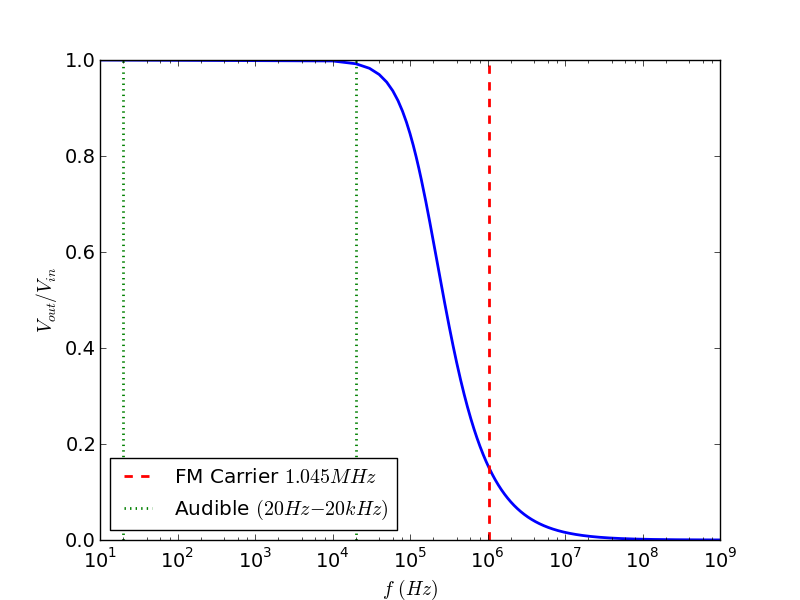
\includegraphics[width=380px]{FM_Reciever_LowPass}
}
\caption{Transfer function of our low-pass filter for $R =1k\Omega$, $C=1nF$, and a roll-off of $160kHz$. This filter will essentially average out the high frequencies of the carrier wave (red dotted line) while leaving frequencies in the audible range unattenuated (green dotted lines).}
\label{fig:lowpasstransfer}
\end{figure}

\subsubsection*{Building the Amplifier}
For the amplifier, we want a gain of at least 2. We choose values for the base and collector resistors such that we will have a gain of 2 for DC signals (and a larger gain for AC signals), using Eq.\ref{amplifiergain}. 
\begin{center}
  \begin{tabular}{ c  c }
    $R_{collector}$ & $270\Omega$ \\
    $R_{emitter}$ & $104\Omega$  \\
    $C_{emitter}$ & $100\mu F$\\
  \end{tabular}
\end{center}
This should give us a gain of $g=2.6$ for DC signals, and greater gain for AC signals due to the capacitor in parallel with $R_{emitter}$.

To choose the values of the biasing resistors, we need to consider the current we want flowing through the transistor. We wanted about $1mA$ of current flowing through, so using Eq.\ref{eq:setcurrent} we chose the biasing resistors to be $1.5k\Omega$ and $300\Omega$. With our power supply at $5.6V$, our base will be biased at $0.93V$; thus the current in through $R_{emitter}$ will be centered at $3mA$. Close enough.

\subsubsection*{Building the Emitter-Follower}
For the emitter-follower, we choose biasing resistors of equal value, so that the biasing will be centered halfway between the power source and GND. Because of the limits on the signal at the base described in Eqs. \ref{eq:maxbase} and \ref{eq:minbase}, centering $V_{base}$ at $V_{powersource}/2=+2.8V$ will allow us to handle the largest signals possible.

We picked two $15k\Omega$ biasing resistors for this purpose, making sure they were large so that the biasing circuit would not draw significant current from the other branch. We then verify that the maximum amplitude signal that this configuration can handle before deing distorted is $2.2V$ (spoiler alert: its true).

As for the emitter resistor, we again choose a value that would give us approximately $1mA$ through the emitter resistor: Our choice of $R_{emitter}=2.2k\Omega$ will give us current centered about $1.2mA$.

\subsection*{Measuring Impedance and Terminating a Cable}
It is important to properly terminate cables because of reflections at points where the impedance is mismatched. A terminated cable will have no reflections when the impedance of the terminator is equal to the impedance of the cable itself.

To estimate the impedance of the cable, we will begin by sending in a $100kHz$ square wave to a T-connector at the scope input. At the other end of the T-connector, we will connect the very long cable (VLC). What we should see on the scope will look like Figure \ref{fig:reflections}, where the scope trace is the sum of the actual square wave signal and the slightly delayed reflection coming from the open end of the cable.

To determine the impedance of the cable, we will terminate the cable by connecting resistors to the far end of it and observing how it affects the scope trace. If we begin to see inverted reflections, it means our terminator's impedance is too low; if we see uninverted reflections, it means our impedance is too high. We will continue trying different resistors---when the cable is properly terminated, the reflections should disappear and the square wave will be undistorted.

\subsection*{Estimating Cable Length}
To estimate the length of the cable, we will use the same procedure as above to get the scope trace in Figure \ref{fig:reflections}. This time, we will read the time delay between incoming signal and reflected signal off of the scope's x-axis. By using Eq.\ref{eq:cablelength} and estimating the speed of signal propogation in the cable to be $\frac{2}{3}c$, we can estimate $l_{cable}$.

\begin{figure}[H]
\center{
  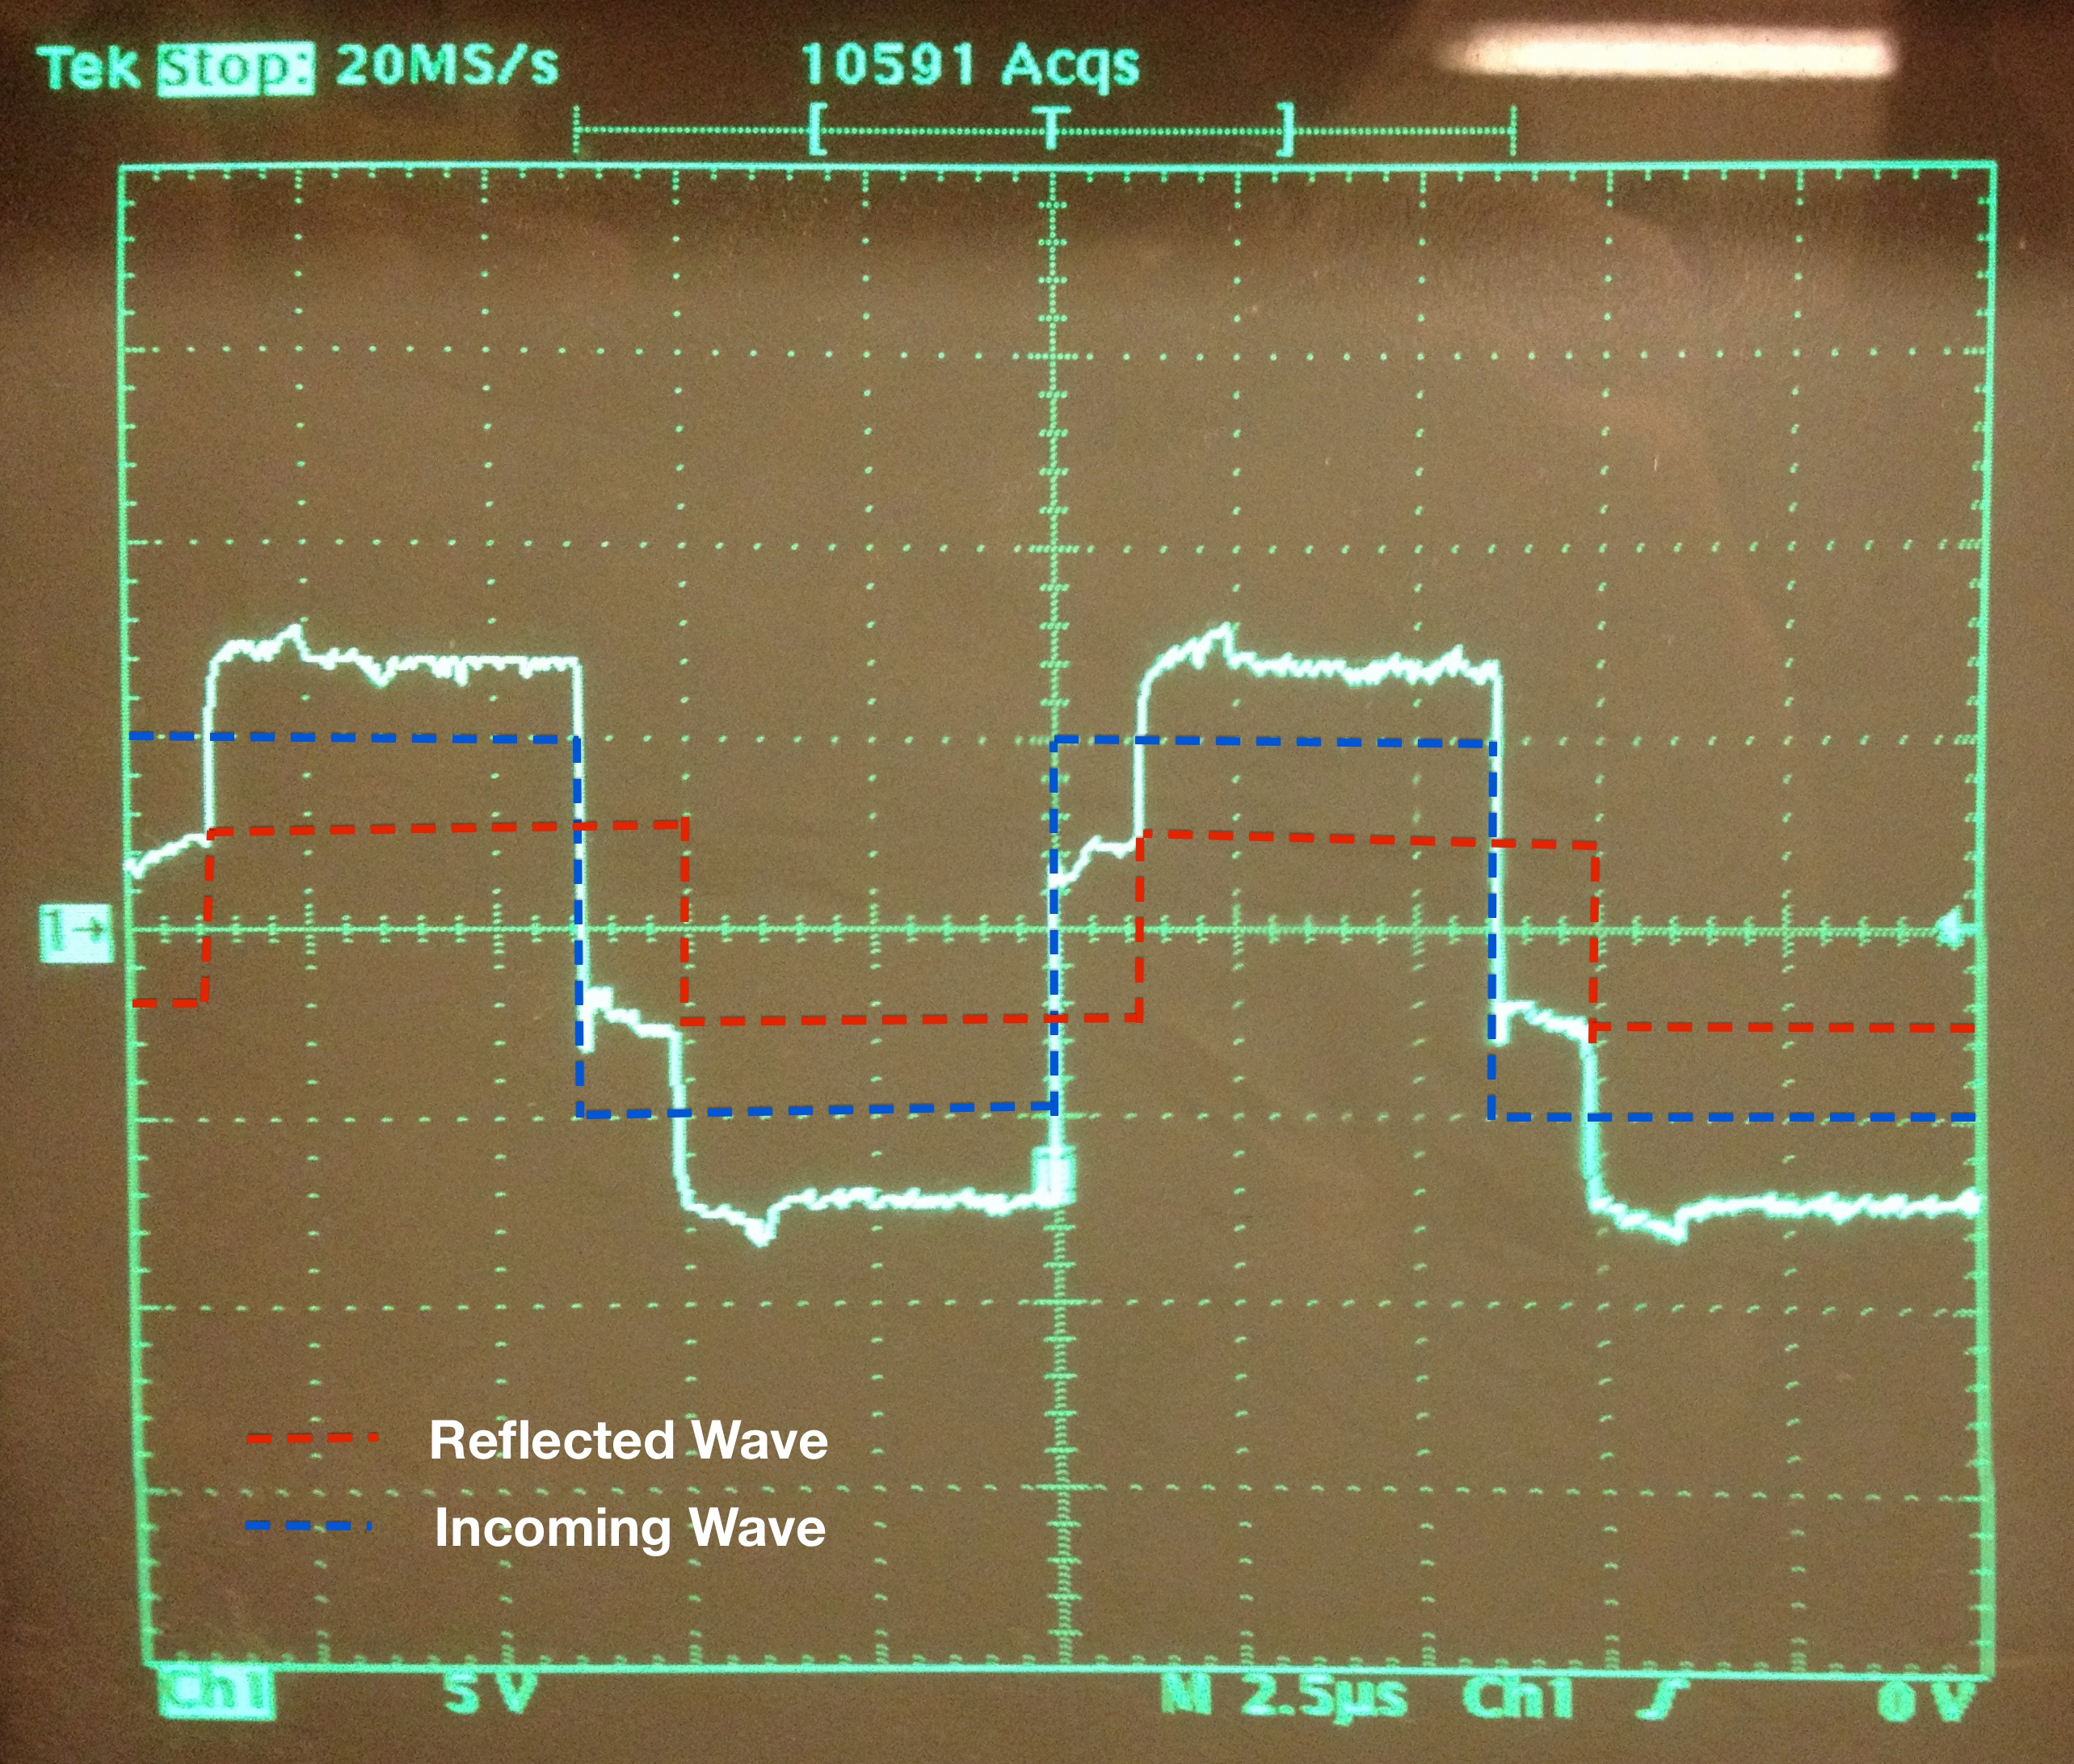
\includegraphics[width=360px]{reflected_signal}
}
\caption[SODUMB]{Scope trace of a $100kHz$ square wave sent down a long cable with no termination. Because the end of the cable is left open, the reflected wave is not inverted and slightly delayed due to the time it takes the signal to travel down the cable and back, and the scope trace shows the sum of the incoming and the reflected waves.}
\label{fig:reflections}
\end{figure}

\subsection*{Noise}
\subsubsection*{Noise Figure}
Unfortunately, the low-noise amplifiers were broken by the time we really understood what we were supposed to do here. Because the Johnson-Nyquist noise ($V=\sqrt{4k_B T B R}$) for a single resistor is on the order of microvolts, we needed at least $\sim 100\times$ gain to be able to estimate the noise on the oscilloscope\footnote{because the thermal noise is so small, using low-noise amplifiers is necessary or the amplifier noise will be overwhelming}.

However, the method to determine an amplifier's noise temperature and noise figure is fairly straightforward: to measure the noise figure of our amplifier, could measure the RMS output voltage of the circuit without an input attached. We would then chain a couple of the low-noise amplifiers in order to get the noise to a measureable level oscilloscope. Knowing the noise voltage and the output impedance of the amplifier, we can use Eq.\ref{johnsonnyquist} to determine the noise temperature and Eq.\ref{eq:noisefigure} to get the amplifier's NF.

\subsubsection*{Central Limit Theorem}
To test and demontstrate the Central Limit Theorem, we will write a program to simulate sampling from random, non-gaussian distributions. By running this a large amount of times, $N$, we will show that the distribution of sampled means is gaussian. To do this I will be interested in the average value of $n=100$ measurements of a random variable---in this case, I will be interested in the average starting value of 100 Blackjack hands\footnote{I will count Aces as 11 unless the sum of the two cards is greater than 21, in which case I count the aces as 1; i.e. the hand AA is worth 12 points).}. By the Law of Large Numbers, the more we make this measurement, the more our results will approach their true distribution; in this case, we hope to see a gaussian distribution.

Additionally, we will demonstrate that the standard deviation on a sampled mean decreases as the inverse square root of the number of samples taken, $n$. For this, we will vary the number of measurements per sample (i.e., I will determine the distribution of the average starting value of $n$ blackjack hands, for $n=5,10,50,$ and $100$). By plotting histograms of the results, we should be able to see that the width fo the distribution decreases for larger $n$. If we find the standard deviation at many values of $n$ we should be able to fit a power law to it and verify the CLT, that $\sigma \propto n^{-1/2}$.

The code I wrote and used can be found in my github respository at

 http://github.com/kevinyu/astro121.git

\section*{Results}
\subsection*{Demodulator Bandpass Filter}
Choosing component values in our bandpass filter gave us a little trouble, due to lost factors of $2\pi$ here and there. Every component value is important: if the resonant frequency is too low, or the bandwidth too narrow (resistor too large), the carrier wave frequencies may fall too far down the response curve and the signal may be attenuated too severely. Convesely, if the resonant frequency is too close to the carrier wave center frequency, or the bandwidth too wide (resistor too small), there may not be enough difference in attenuation across the span of FM frequencies to make a good AM signal. The values that we selected in the Methods section worked well and produced a good AM signal that we were able to extract and ultimately hear in the speaker.  
\subsection*{Demodulator Biasing}
One issue we had at first was a flat output coming out of the low-pass at the end of the demodulator, rather than the desired AC signal. After a bit of confusion, we realized it was due to choosing poor values for our biasing resistors. Originally, we had chosen them both to be the same value; Because it is a voltage divider, the bias would have been one half of the power supply voltage, or $2.8V$. As we know, from the Method section, we needed the diode to pass the positive half of the signal but block the negative half of the signal. However, because here our bias was $2.8V$, much greater than the diode ``on" voltage of $0.6V$, the diode will pretty much \textit{always be conducting}. Thus, the low-pass filter averaged out the AM signal entirely and the amplitude information was lost. To fix this, we chose biasing resistors such that the bias voltage would be much closer to $0.6V$, and found that the demodulator was then successful.

\subsection*{Length of the Cable}
To approximate the length of the cable in the lab, we use the procedure described in the Methods section and Eq.\ref{eq:cablelength}. The scope trace, with the sum of the incoming wave and reflected wave, can be seen in Figure \ref{fig:reflections}. As we can see on the scope trace, the reflected wave is delayed by about $1.2\mu s$, and thus the cable length is (assuming the speed of signal propogation in the cable is $\frac{2}{3}c$):
\begin{eqnarray}
l_{cable} \approx 120m \nonumber
\end{eqnarray}
This is a reasonable result, though is only as accurate as the approximation that $c_{cable} \approx \frac{2}{3}c$.

\subsection*{Impedance of the Cable}
To estimate the impedance of the cable, we will try terminating it with different valued resistors until we do not see any reflections. When terminating the cable with a $10\Omega$ resistor, we saw that the reflection was inverted. We had gone too far. We took this to mean that the impedance of the cable was somewhere between $10\Omega$ and $\infty\Omega$, which really narrowed it down for us. Luckily, our next choice of $56\Omega$ turned out to be close enough, and we saw a very nice trace of a square wave on the oscilloscope with no distorting reflections.
\begin{eqnarray}
Z_{cable} \approx 56\Omega \nonumber
\end{eqnarray}

\subsection*{Central Limit Theorem Demonstration}
In Figure \ref{fig:approachgaussian}, we can see that the distribution of a sample mean is approximately gaussian. By the Law of Large Numbers, the larger we make the value of $N$ the closer our measurements will approximate their true distribution. For this demonstration, I measured the average starting value of $n=100$ blackjack hands. As you can see in the figure, at large values of $N$ our results approach a gaussian distribution. This is true even though the distribution of a single measurement is not gaussian.

\begin{figure}[H]
\center{
  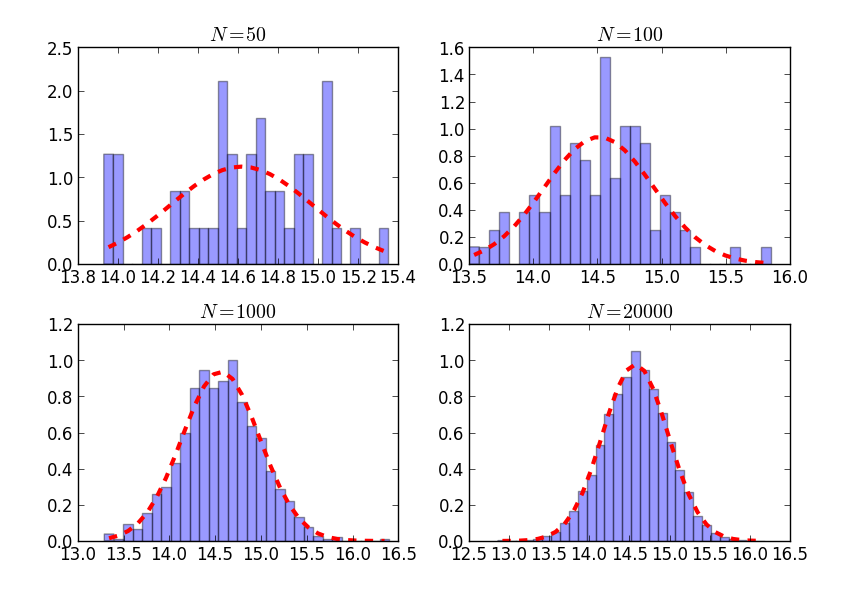
\includegraphics[width=360px]{Blackjack_Gaussian}
}
\caption[SODUMB]{Probability density of the average starting value of $n=100$ blackjack hands. At large $N$, the results should approach their true distribution. The dotted red line is a fitted gaussian to the data.}
\label{fig:approachgaussian}
\end{figure}

\subsubsection*{Allen Variance Test}
To demonstrate the standard deviation's $\frac{1}{\sqrt{n}}$ dependence from Eq.\ref{eq:rootn}, I sampled the average value of $n$ randomly chosen blackjack hands, for sample sizes $n$ ranging from 1 to 10000. For each value of $n$, I recorded the standard deviation of $N=20$ measurements of the mean. Figure \ref{fig:n_scaling} visually demonstrates the narrowing of the distributions for large $n$, while Figure \ref{fig:n_scaling2} demonstrates the relationship in Eq.\ref{eq:rootn}. Our data suggests that
\begin{eqnarray}
\sigma \propto n^{-0.51 \pm 0.21} \nonumber
\end{eqnarray}
which is in close agreement with the CLT. If this were the noise output of our amplifier, this agreement would demonstrate that the noise is random and not systematic. 
\begin{figure}[H]
\center{
  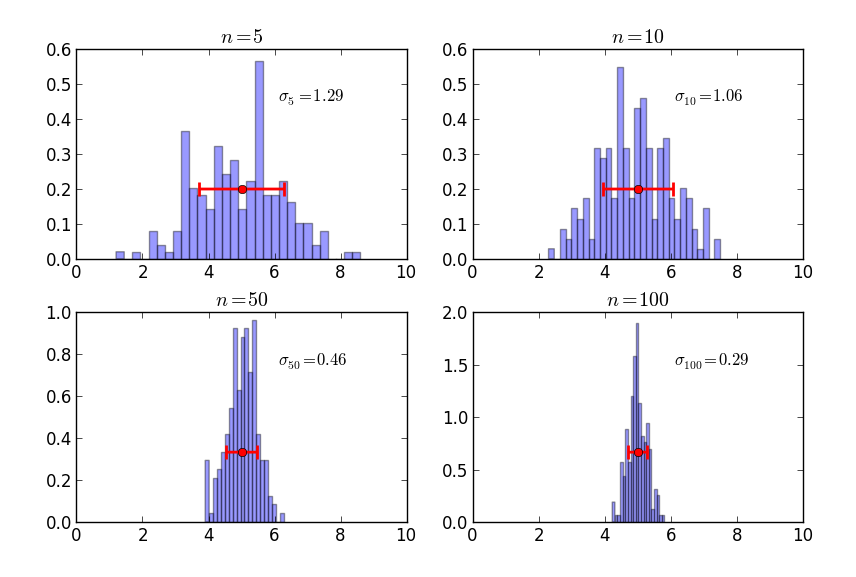
\includegraphics[width=340px]{CLT_n_scaling}
}
\caption[SODUMB]{The standard deviation of $N=20$ measurements of samples of size $n$, for $n=5,10,50,100$. As you can see, the width of the distribution decreases as $n$ increases. Note that all four histograms have the same scale on the x-axis.}
\label{fig:n_scaling}
\end{figure}
\begin{figure}[H]
\center{
  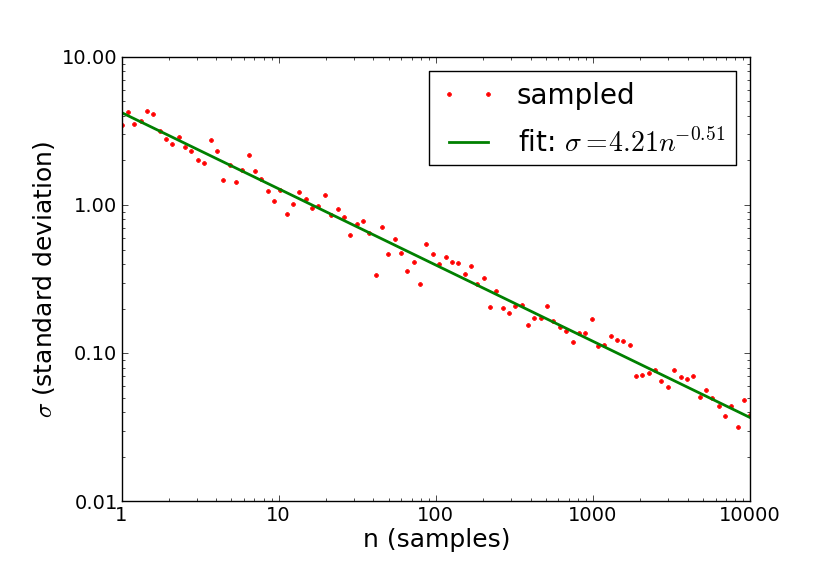
\includegraphics[width=340px]{CLT_sigma_vs_n}
}
\caption[SODUMB]{The relationship between the sampled standard deviation, $\sigma$, and the number of samples in each measurement, $n$, visualized on a log-log plot. It is clear that the data approximately follows a $n^{-1/2}$ rule, as a least-squares fit returned a power relationship of $\sigma \propto n^{-0.51\pm0.02}$. This is an example of an Allen Variance Test.}
\label{fig:n_scaling2}
\end{figure}

\section*{Conclusion}
Our assembly of a FM receiver circuit was successful, and we were able to connect it to a speaker and hear the output. In order to do so, we utilized many basic tools of analog circuits: a LC Bandpass filter to differentiate the input, a diode and low-pass filter to detect the signal envelope, and amplifier to increase the amplitude of our signal, and a follower to match output and input impedances between the rest of the circuit and the low-impedance speaker.

Our understanding of RC and LC filters, especially using capacitors to ``slow" the response of a circuit, should be a useful tool in the future when wanting to isolate a signal of interest from background noise and unwanted interference. Additionally, understanding amplifiers and how amplifiers propogate noise will certainly be important when trying to make measurements on small signals.

Finally, understanding the statistical characteristics of random noise using the CLT will be important because almost all measurements will have some inherent statistical variations. This can be caused by a variety of factors, including hardware limitation and the signal quality. This is especially true when trying to detect relatively small signals, when the signal to noise ratio may be less than ideal. By averaging many samples, however, random noise can be removed (since the variance of the measurement decreases linearly with the number of samples averaged), resulting in better data.

\section*{Acknowledgement}
I would like to thank my lab parters, Jeff Lievense and Maissa Salama, for working hard in getting through this lab with me. I wonder if you guys will actually read the acknowledgement, but I also appreciate the work and help of the lab instructors---Prof. Aaron Parsons, Karto Keating, and Baylee Bordwell---for making the lab possible to complete, despite the pain it has caused us all.
All figures were done in Python using the Numpy and Matplotlib libraries.
Except for the voltage divider, my circuit diagrams were created in LTSpice, which is free, so at least it has that going for it.

\end{document}